% vim: ts=2:sw=2:tw=80:et
This manual describes the use and operation of Arbwave, the arbitrary waveform
experimental control program.

\section{What is Arbwave?\index{What is Arbwave?}}

\section{What can Arbwave do?}

We can also refer to a figure as Fig.~\ref{fig:intro:jdk_grid_example}.

\begin{figure}[hb]
    \centerline{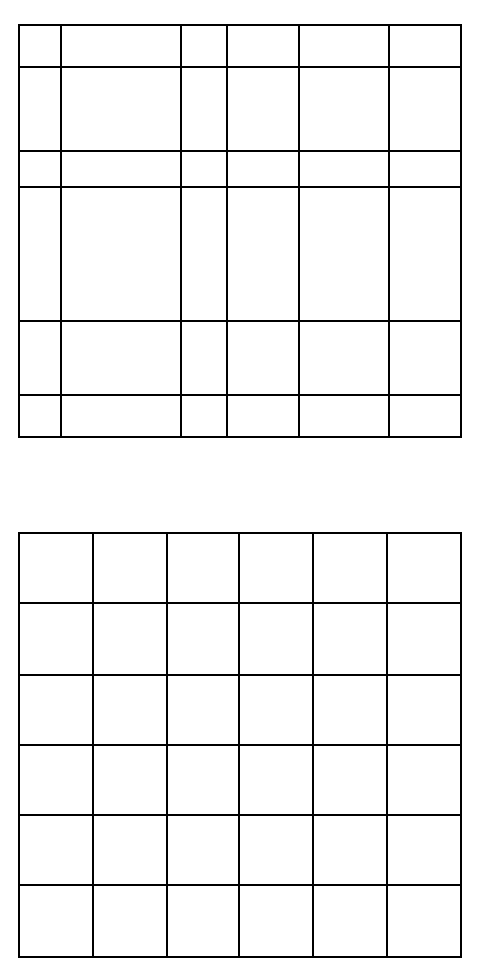
\includegraphics[angle=-90]{figures/jdk_grid_example}}
    \caption{Regular mesh on the left; stretched mesh, in both directions, on
             the right.} 
    \label{fig:intro:jdk_grid_example}
\end{figure}

We just love to cite \citet{Rambo:1989}.
